%%%%           %%%%
%%%% ANÁLISIS  %%%%
%%%%           %%%%

\chapter{Análisis}
\label{chap:analisis}

\lettrine{E}{n} este capítulo se tratará los aspectos del análisis de la aplicación. Se verán los requisitos, funcionales y no funcionales, los casos de uso y por último se presentarán los modelos de los documentos tratados.

\section{Actores y casos de uso}

Un caso de uso describe una interacción en entre un rol y el sistema. O cómo es utilizado por un usuario para completar una tarea u alcanzar un objetivo. En el diagrama \ref{fig:casos-de-uso} se presentan los casos de uso de la aplicación. 

Existen dos actores que interactúan con la aplicación, un sistema externo y una base de datos:

\begin{itemize}
	\item \textbf{Sistema externo}: la aplicación está diseñada para comunicarse con sistemas externo mediante invocación directa de comandos o bien un API REST. Si bien mediante comandos un usuario podrían solicitar la ejecución de trabajos en el engine, el objetivo principal es ser un backend conectado empleado por otros sistemas.
	\item \textbf{Base de datos}: este agente es consultado para la obtención de datos de idenficación de los documentos.
\end{itemize}

Se presentan a continuación los casos de uso de forma detallada:

\begin{itemize}
	\item \textbf{CU-01} - Registrar nuevo trabajo
	\begin{itemize}
		\item \textbf{Descripción}: el sistema externo solicita la generación de un nuevo identificador para un trabajo.
		\item \textbf{Precondición}: el motor está operativo y esperando trabajo.
		\item \textbf{Postcondición}: se genera el identificador y se ha creado la ruta correspondiente en el sistema de ficheros para el trabajo.
	\end{itemize}
\item \textbf{CU-02} - Generar JSON
	\begin{itemize}
		\item \textbf{Descripción}: el sistema externo facilita un lote de ficheros y un identificador del trabajo para comenzar su tratamiento.
		\item \textbf{Precondición} el identificador debió ser creado previamente.
		\item \textbf{Postcondición}: los resultados de la operativa están disponibles en las rutas previstas.
\end{itemize}
\item \textbf{CU-03} - Generar imágenes
	\begin{itemize}
		\item \textbf{Descripción}: el sistema genera imágenes para cada una de las páginas de los documentos.
		\item \textbf{Precondición} se han podido recuperar los PDF individuales y se encuentran en las rutas previstas.
		\item \textbf{Postcondición}: existe un fichero para cada página de cada documento.
\end{itemize}
\item \textbf{CU-04} - Informar error
	\begin{itemize}
		\item \textbf{Descripción}: en caso de problemas durante el procesamiento se informa al sistema externo del error ocurrido.
		\item \textbf{Precondición} sucece una condición de error en el sistema.
		\item \textbf{Postcondición}: dependiendo del tipo de error el engine consigue finalizar el procesamiento o se finaliza si no es posible recuperarse del error.
\end{itemize}
\item \textbf{CU-05} - Relacionar documento y plantilla
	\begin{itemize}
		\item \textbf{Descripción}: a partir de los datos extraídos del documento en curso se consigue identificar la plantilla correcta para la generación de su lenguaje intermedio y su posterior proceso de parseo. La búsqueda del identificador se solicita a una base de datos externa.
		\item \textbf{Precondición} los datos extraidos son de la suficiente calidad para contener el identificador del documento.
		\item \textbf{Postcondición}: se genera un fichero con el identificador único de la plantilla.Precondición
\end{itemize}
\item \textbf{CU-06} - Identificar la finalización
	\begin{itemize}
		\item \textbf{Descripción}: al finalizar el procesamiento del lote de ficheros se genera una marca de finalización del trabajo.
		\item \textbf{Precondición} se completa el tratamiento de todos los documentos sin errores mayores.
		\item \textbf{Postcondición}: la marca de finalización está en la ruta preestablecida del sistema de ficheros.
\end{itemize}

\end{itemize}

\begin{figure}[hp!]
	\centering
	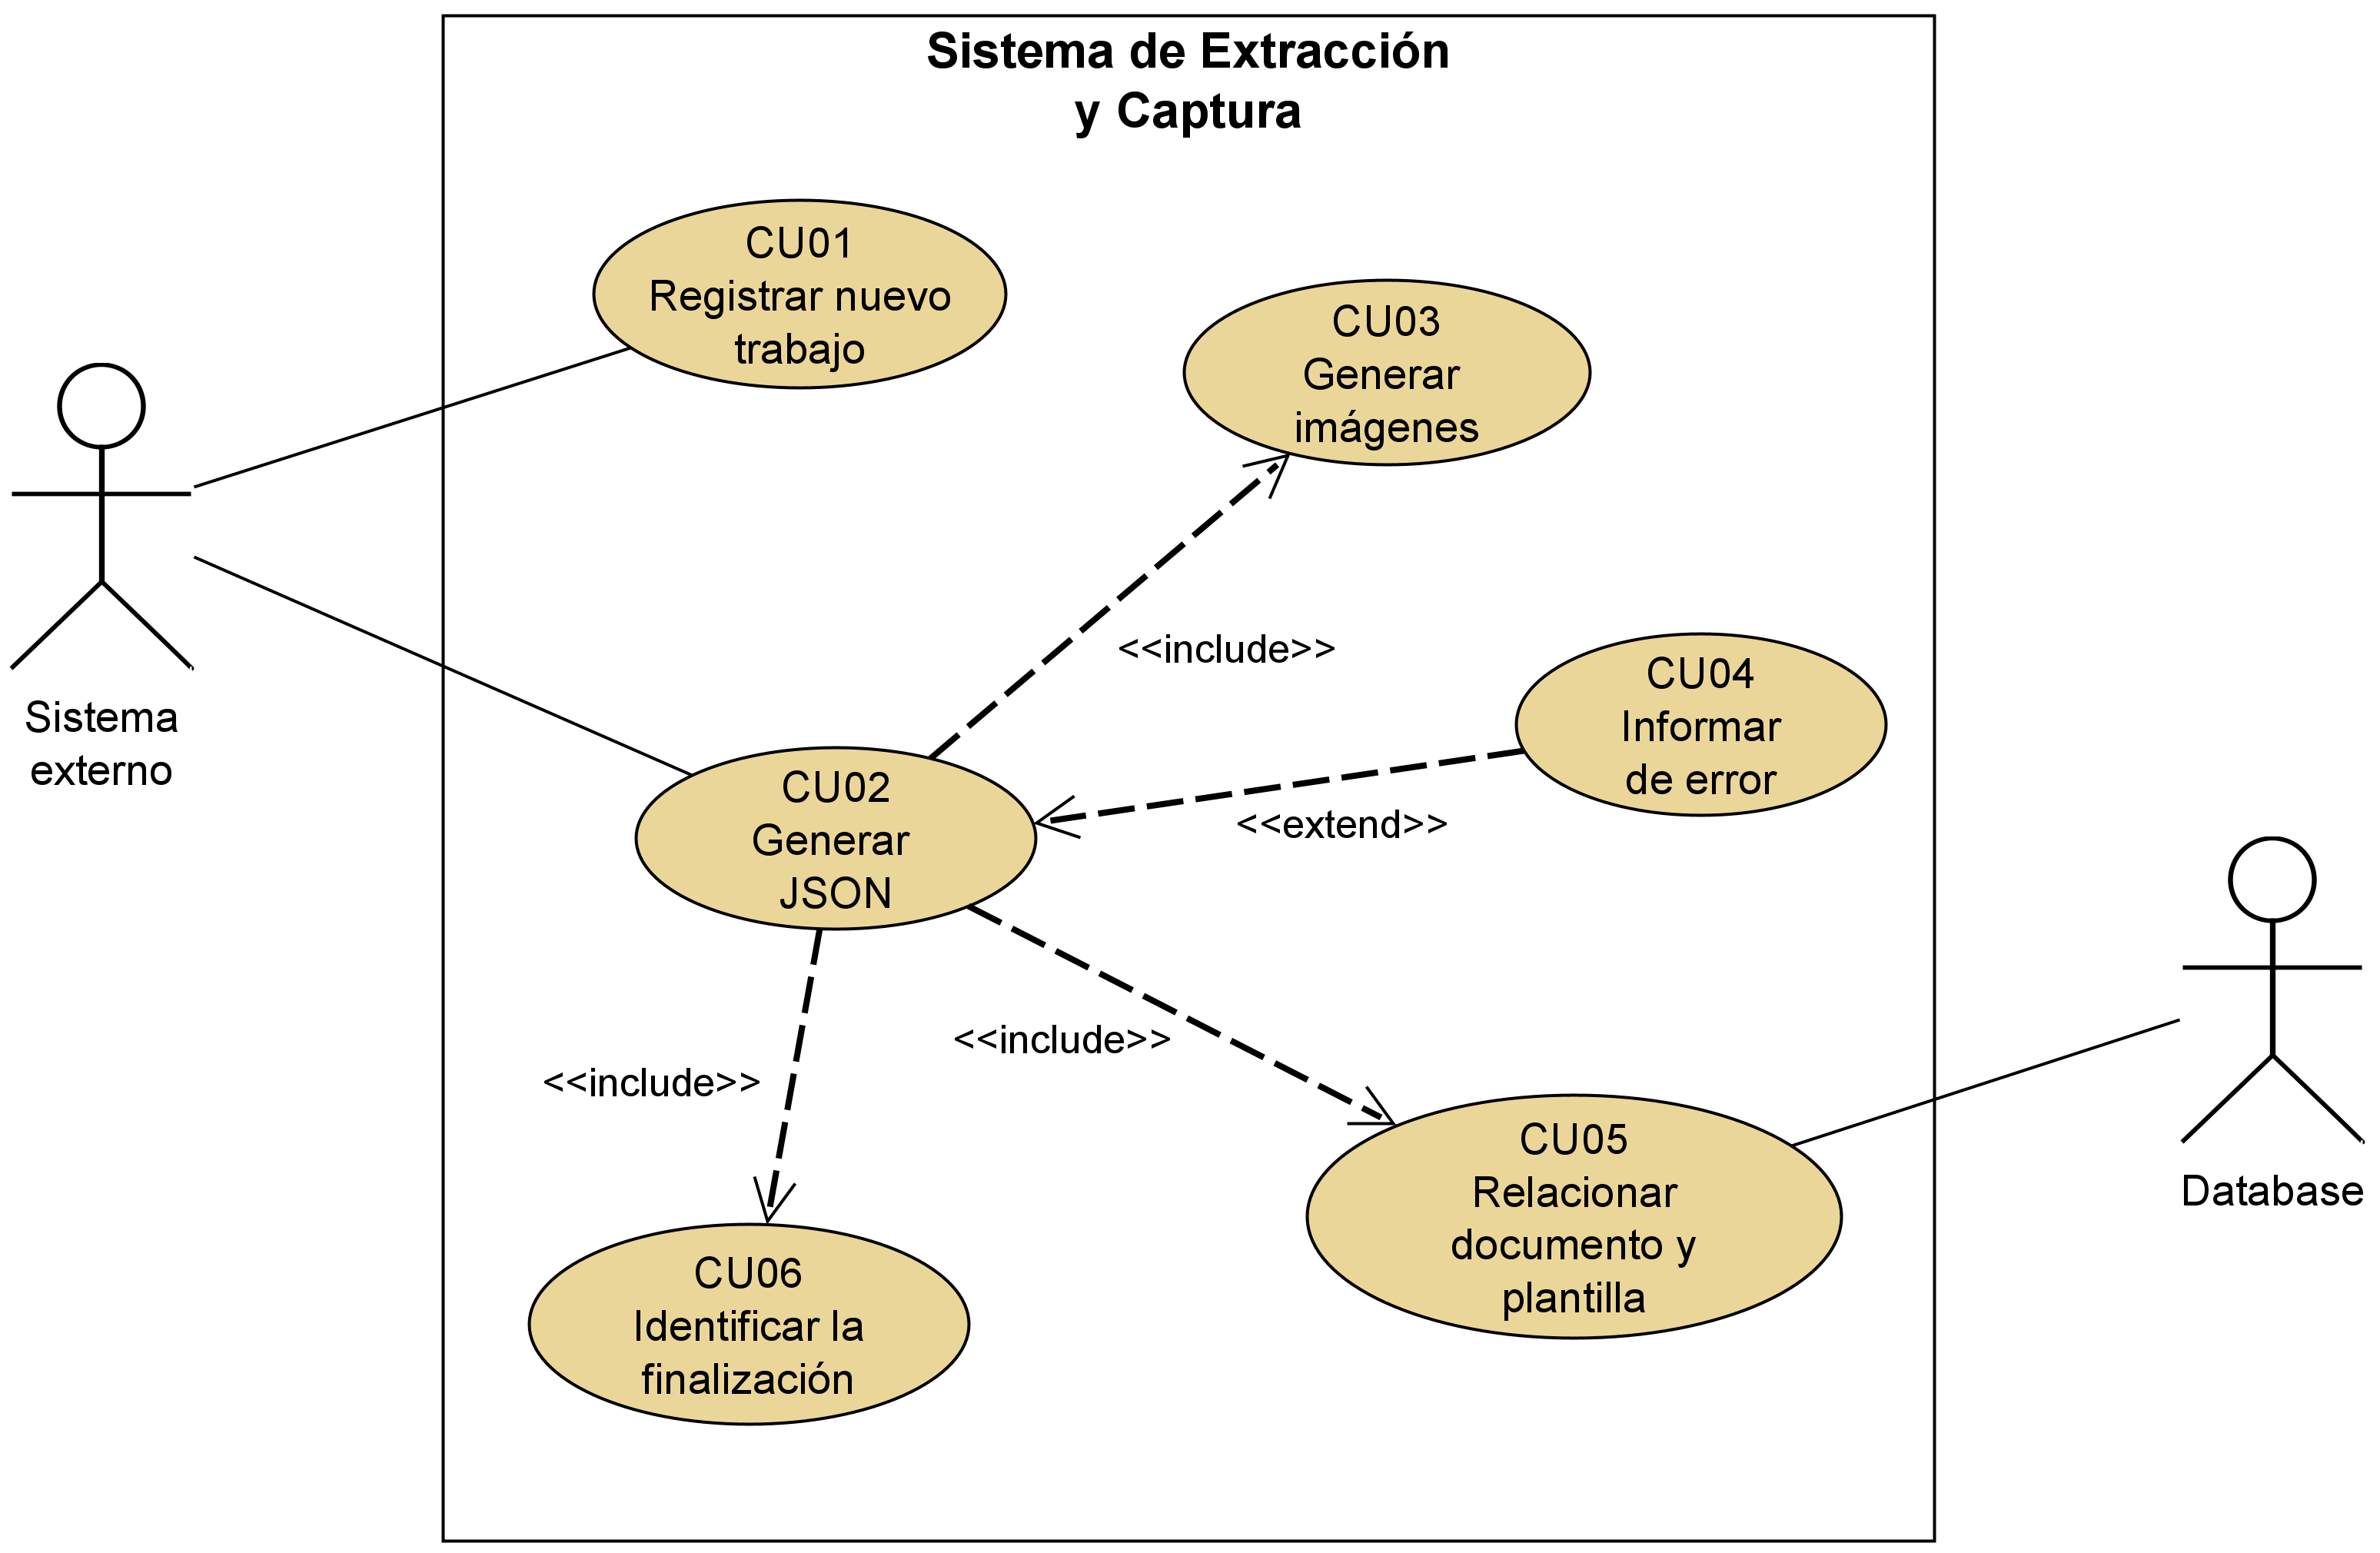
\includegraphics[width=1.0\textwidth]{imaxes/g-analisis/casos-uso.png}
	\caption{Casos de uso de la aplicación}
	\label{fig:casos-de-uso}
\end{figure}

\section{Requisitos funcionales}

\section{Requisitos no funcionales}

\section{Sobre los documentos}

\subsection{Tipos de regiones}

\subsection{Características para la identificación}

Datos para identificar los documentos. En este caso, NIF, CIF.

% TODO valorar si comentar los distintos tipos de lineas presentes en los documentos

%%%%%%%%%

\begin{itemize}
	\item El sistema debe ser capaz de recepcionar 1 o múltiples ficheros por petición
	\item El sistema debe ser capaz de tratar cada uno de los ficheros de forma independiente y generar su propia salida
	\item El sistema debe ser capaz de tratar ficheros basados en texto o imagen
	\item El sistema debe ser capaz de generar una salida en formato estructurado
	\item El sistema debe ser capaz de generar imágenes de las páginas del documentos para disponibilidad del frontend
	\item El sistema debe ser capaz de generar un identificador único para cada trabajo tratado
	\item El sistema debe ser capaz de generar una marca indicativa del final de procesamiento
	\item El sistema debe ser capaz de identificar líneas individuales en las tablas de los documentos. Aquí se puede hablar de por que
\end{itemize}

\begin{itemize}
	\item Mantener reducido el tiempo de cómputo    
\end{itemize}
